\section{Data Approximation}
\label{sec-data}






Big data has large volume, and, hence, the space complexity~\cite{CormenLRS01} of big data analytic tasks starts raising more concerns.
Given a class $Q$ of queries on data $D$, data approximation is to transform $D$ into smaller $D'$ such that $Q$ on $D'$ returns a sufficient or satisfiable approximate answer in a more efficient way. Further, it is typically common that query $Q$ needs to be (slightly) modified to $Q'$ to accommodate  the changes of $D$ to $D'$, as shown in Fig.~\ref{fig-tech-dataappro}. Similar to query approximation, data approximation needs to reach a balance between the query efficiency and answer quality.


The rationale behind data approximation has roots in the Pareto principle\footnote{\small \url{https://en.wikipedia.org/wiki/Pareto_principle}} that ``states that, for many events, roughly 80\% of the effects come from 20\% of the causes''. The critical thing for data approximation is to determine which part of data is relevant to tasks (belong to the 20\%).
 By this principle, for many big analytic tasks, one may only need to keep a small amount of the data to derive high quality answers.
For example, when we are to build a predictive model on the stock of razers for an online store based on the order history of customers, orders from men are good enough. While on the stock of lipsticks, those from women are good enough. That is to say,  it is not necessary to use the entire data for certain data analytic tasks.



However, it should be pointed out that there are data analytic tasks such that data approximation could not work well. For example, an online store needs to count the total number of goods in its catalog.  Essentially entire goods should be considered for this task, and if a (small) portion of goods are chosen, it is hard to have a satisfiable result.


We next explain data approximation computation in more detail using three different data analytic tasks.



\stitle{(1) Proxies for Shortest Paths and Distances~\cite{MaFLWCH16}}. Computing shortest paths and distances is one of the fundamental problems on graphs. We study the {\em node-to-node shortest path} ({\em distance}) problem on large graphs: given a weighted undirected graph $G(V, E)$ with non-negative edge weights, and two nodes of $G$, the source $s$ and the target $t$, find the shortest path (distance) from $s$ to $t$ in $G$. The Dijkstra's algorithm with Fibonacci heaps runs in $O(n\log n + m)$ due to Fredman \& Tarjan~\cite{CormenLRS01}, where $n$ and $m$ denote the numbers of nodes and edges in a graph, respectively, which remains asymptotically the fastest known solution on arbitrary undirected graphs with non-negative edge weights.
%The challenge of computing shortest paths on large graphs.
However, computing shortest  paths and distances remains a challenging problem, in terms of both time and space cost, on large-scale graphs. Hence, various optimizations have been developed to speed-up the computation.

To speed-up shortest  path and distance queries, we propose {\em proxies} that have the following properties:
%
(a) each proxy captures a set of nodes in a graph, referred to as \dra,
%
(b) a small number of proxies can represent a large number of nodes in a graph,
%
(c) shortest paths and distances involved within the set of nodes being represented by the same proxies can be answered efficiently, and,
%
(d) the proxies and the set of nodes being represented can be computed efficiently in {\em linear} time.



The framework for speeding-up shortest path and distance queries with proxies consists of modules preprocessing and query answering as follows.


\ni(a) {\em Preprocessing}: Given graph $G(V, E)$, it first computes all \dras and their maximal proxies in linear time, then it computes and stores all the shortest paths and distances between any node and its proxy. It finally computes the reduced subgraph $G'$ by removing all \dras from graph $G$, \ie keeping the proxies only.


\ni(b) {\em Query answering}. Given two nodes $s$ and $t$ in graph $G(V$, $E)$  and the pre-computed information above, the query answering module essentially executes the following.

The shortest path $\path(s, t)$ = $\path(s, u_s)/$ $\path(u_s, u_t)/$ $\path(u_t, t)$, where $u_s$ and $u_t$ are the proxies of $s$ and $t$, respectively.
Here  $\path(s, u_s)$ and $\path(u_t, t)$ are pre-computed, and $\path(u_s, u_t)$ can be computed on the reduced subgraph $G'$ by invoking any existing algorithms
(\eg \ah~\cite{zhu2013shortest}).
%
The shortest distance $\dist(s, t)$ = $\dist(s, u_s)$ + $\dist(u_s, u_t)$ + $\dist(u_t, t)$ can be computed along the same line.

We show experimentally show that about $1/3$  nodes of real-life social networks and road networks  are captured by proxies, leaving $2/3$ in the reduced graphs.
Essentially, we propose a light-weight data reduction technique for speeding-up (exact)  shortest path and distance queries on large weighted undirected graphs~\cite{MaFLWCH16}.




\begin{figure}[tb!]
  \vspace{-1ex}
  \begin{center}
  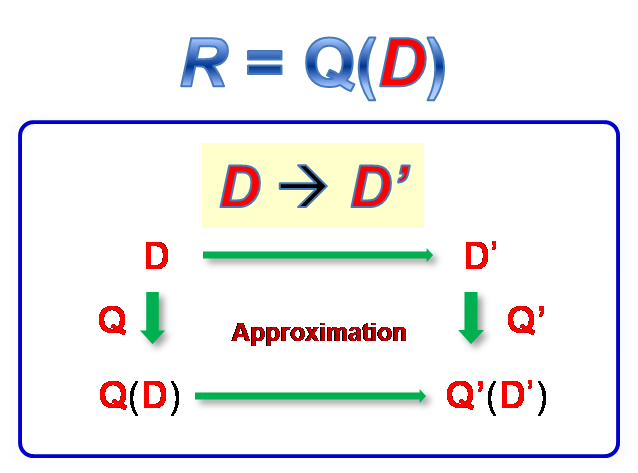
\includegraphics[scale=0.5]{./dataApprox.png}
  \end{center}
  \vspace{-3ex}
  \caption{Data approximation}\label{fig-tech-dataappro}
  \vspace{-2ex}
\end{figure}

\stitle{(2) Ensemble Enabled Link Prediction~\cite{DuanMAMH17}}. Link prediction is the task to predict the formation of future links in a dynamic and evolving network, and has been extensively studied due to its numerous applications, such as the recommendation of friends in a social network, images in a multimedia network, or
collaborators in a scientific network.


Link prediction methods are often applied to very large and sparse networks, which has a large {\em search space} $O(n^2)$,
where $n$ is the number of nodes. Hence, the scalability is a big challenge. In fact, an often overlooked fact is that most {\em exiting link prediction algorithms evaluate the link propensities only over a subset of possibilities rather than all propensities over the entire network},
\eg \cite{zhu2016}..
In order to understand why this is the case, consider a large network with $10^8$ nodes. Its number of {\em possibilities} for links
is of the order of $10^{16}$. Therefore, a 3GHz processor would
require at least $35$ days just to allocate one {\em machine cycle} to
every pair of nodes. This implies that in order to determine the
top-ranked link predictions over the {\em entire network}, the
running time will be much much larger than $35$ days.

It is noteworthy that most existing link prediction algorithms are not designed to search over the entire
$O(n^2)$ possibilities. A closer examination of the relevant
studies shows that even for networks of modest size, these
algorithms perform benchmark evaluations over a {\em
sample of the possibilities} for links.  In other
words, the {\em complete ranking problem for link prediction in
very large networks remains challenging at least from a
computational point of view}.


Latent factor models have been shown to be wildly successful in the domain of
collaborative filtering, but not link prediction in spite of the obvious
similarity between link prediction and collaborative filtering and
the obvious effectiveness of latent factor models. One of the reasons why latent factor models are rarely used for
link prediction is due to their complexity. In
collaborative filtering applications, the item dimension is of the
order of a few hundred thousand, whereas even the smallest  real-world networks contain more than a million nodes.
Even worse, we also experientially find that the quality of link prediction for latent factor models decreases with the increase of data sparsity,
and networks typically become sparser when their sizes grow larger.




\eat{%%%%%%%

The factorization of a matrix of
size $O(n^2)$ is not only computationally expensive, but also
memory-intensive.  As will be seen later in this article, one advantage
of  latent-factor models is that they are able to  transform the
adjacency matrix to a multidimensional space which can be searched
efficiently {\em by pruning} large portions of the $O(n^2)$ search
space in order to recommend the top-$k$ possibilities.

\begin{table}
\caption{The $O(n^2)$ problem in link prediction: Time required to
allocate a {\em single machine cycle} to every node-pair possibility
in networks of varying sizes and processors of various speeds.}
\label{time}
\vspace{0ex}
\centering
\begin{tabular}{cccc}
\hline \hline Network Sizes & 1 GHz &  3 GHz & 10 GHz \\
\hline \hline $10^6$ nodes & 1000 sec. & 333 sec. & 100 sec.\\
\hline $10^7$ nodes & 27.8 hrs &  9.3 hrs &  2.78 hrs\\
\hline $10^8$ nodes & $>100$ days &  $>35$ days & $> 10$ days\\
\hline $10^9$ nodes & $>10000$ days & $>3500$ days & $> 1000$ days\\
\hline \hline
\end{tabular}
\vspace{-2ex}
\end{table}
}%%%%%%%%%%%


We explore an {\em ensemble approach} to making latent factor models
practical for link prediction by decomposing the search space into a
 set of smaller matrices with three structural bagging methods with performance guarantees, which has obvious {\em
effectiveness} advantages. In this way, latent factor models only need to deal with networks with small sizes (and denser), and retain
their effectiveness and efficiency.  By incorporating with the characteristics of  link prediction, the bagging methods maintain high prediction
accuracy while reducing the network size via graph sampling techniques.
Further, the same bias-variance tradeoffs apply to the link-prediction problem, as the
standard classification problem. Therefore, the use of an ensemble
approach has obvious robustness advantages as well.


We experimentally show that our ensemble approach is over $50$ times faster and  over $20\%$ more accurate than {\sc bigclam} \cite{yang-wsdm2013} on using real-life social networks.


\eat{
\stitle{(1) Network Anomaly Detection~\cite{HuAMH16}}
We have adopted the idea in the process of dealing with large graphs in the study of anomaly detection in graph streams, when dealing with the matrix representation of a social graph, and  we have both theoretically and experimentally shown that simplifying the matrix by replacing a part of small entry values  with zero has few affects on the computation of eigenvectors~\cite{YuAMW13}.
}%%%%%%%%%%%%EAT






